%\title{emnlp 2017 instructions}
% File emnlp2017.tex
%

\documentclass[11pt,letterpaper]{article}
\usepackage{emnlp2017}
\usepackage{times}
\usepackage{latexsym}
\usepackage{graphicx}
\usepackage{amssymb}
\usepackage{amsmath}
\usepackage{multirow}

% Uncomment this line for the final submission:
\emnlpfinalcopy

%  Enter the EMNLP Paper ID here:
% \def\emnlppaperid{***}

% To expand the titlebox for more authors, uncomment
% below and set accordingly.
% \addtolength\titlebox{.5in}    

\newcommand\BibTeX{B{\sc ib}\TeX}

\title{Discovering Cognates Using LSTM Networks}

% Author information can be set in various styles:
% For several authors from the same institution:
% \author{Author 1 \and ... \and Author n \\
%         Address line \\ ... \\ Address line}
% if the names do not fit well on one line use
%         Author 1 \\ {\bf Author 2} \\ ... \\ {\bf Author n} \\
% For authors from different institutions:
% \author{Author 1 \\ Address line \\  ... \\ Address line
%         \And  ... \And
%         Author n \\ Address line \\ ... \\ Address line}
% To start a seperate ``row'' of authors use \AND, as in
% \author{Author 1 \\ Address line \\  ... \\ Address line
%         \AND
%         Author 2 \\ Address line \\ ... \\ Address line \And
%         Author 3 \\ Address line \\ ... \\ Address line}
% If the title and author information does not fit in the area allocated,
% place \setlength\titlebox{<new height>} right after
% at the top, where <new height> can be something larger than 2.25in
\author{Shantanu Kumar \and Ashwini Vaidya \and Sumeet Agarwal \\ 
  Indian Institute of Technology Delhi
  \\ {\tt \{ee1130798, ird11278, sumeet\}@iitd.ac.in}}

\date{}

\begin{document}

\maketitle

%%%%%%%%%%%%%%%%%%%%%%%%%%%%%%%%%%%%%%%%%%%%%%%%
\begin{abstract}
In this paper, we present a deep learning (DL) model for the task of pairwise cognate prediction. We use a character level model with recurrent neural network architecture and attention. We compare the performance of our model with previous approaches on various language families. We are able to show that our model performs better than non-DL methods which exploit surface similarity measures as well as a recent convolutional neural network (CNN) based model for the task.
\end{abstract}

%%%%%%%%%%%%%%%%%%%%%%%%%%%%%%%%%%%%%%%%%%%%%%%%
\section{Introduction}
Cognates are words across different languages that are known to have originated from the same word in a common ancestral language. For example, the English word `\textit{Night}' and the German word `\textit{Nacht}', both meaning \textit{Night} as well as the English `\textit{Hound}' and German `\textit{Hund}', meaning \textit{Dog} are cognate word pairs, whose origin can be traced back to Proto-Germanic.

Traditionally, the identification of cognates was carried out by historical linguists, using word lists and establishing sound correspondences between words. These are useful in determining linguistic distance within a language family, and also to understand the process of language change. Cognate information has also been used in several downstream NLP tasks, like sentence alignment in bi-texts \cite{simard1993using} and improving statistical machine translation models \cite{kondrak2003cognates}. Additionally, it has been proposed that cognates can be used to share lexical resources among languages that are closely related \cite{Singh:07b}.

For some time now, there has been a growing interest in automatic cognate identification techniques. Most approaches for this task focus on finding similarity measures between a pair of words such as orthographic or phonetic similarity \cite{hauer2011clustering} \cite{inkpen2005similarity} \cite{List2016g}. These are used as features for a classifier to identify cognacy between a given word-pair. Surface similarity measures miss out on capturing generalizations beyond string similarity, as cognate words are not always revealingly similar. \citet{rama2015automatic} attempt to identify cognates by looking at the common subsequences present in the candidate word pair. For a cognate pair like the English `\textit{Wheel}' and the Sanskrit `\textit{Chakra}', such an approach fails as there are no letters in common. In fact, even for a pair like English `\textit{Father}' and Latin `\textit{Pater}', a common subsequence approach completely ignores the similarity between the `\textit{Fa}' and `\textit{Pa}' phonemes, which is a possible indication of cognacy between the pair. Thus, there is a need of information about phonological similarity that is beyond surface similarity, such as the sound correspondences that are used in historical linguistics to narrow down candidate pairs as cognates.

By using DL based models, the need for external feature engineering is circumvented as the system learns to find hidden representations of the input depending on the task in hand. Our paper presents an end-to-end character-level recurrent neural network (RNN) based model that is adapted from a model used on a similar word-level task called RTE \cite{rocktaschel2016reasoning}. Our model is able to outperform both the common subsequence model \cite{rama2015automatic} as well as a recent CNN-based model \cite{rama2016siamese} on the task. 

%%%%%%%%%%%%%%%%%%%%%%%%%%%%%%%%%%%%%%%%%%%%%%%%
% \section{Related Work}

% There have been several previous works for automatic cognate identification that try to exploit different forms of features and representations for capturing the necessary information.

% \textbf{Orthographic features based classifier} : \cite{hauer2011clustering} use a number of basic word similarity measures as input to a SVM classifier for cognate prediction. They use features like common bigrams, longest common substring, word length difference etc. The also use features that encode the degree of affinity between pairs of languages.

% \textbf{Gap-weighted common subsequences} : \cite{rama2015automatic} uses a string kernel based approach wherein he defines a vector for a word pair using all common subsequences between them and weighting the subsequence by their gaps in the strings. The subsequence based features outperform orthographic word similarity measures.

% \textbf{Siamese ConvNet model} : In a recent work, T. Rama introduces CNN based siamese-style model \cite{rama2016siamese} for the task. The model is inspired by image-similarity CNN models. Instead of CNNs, we propose the use of LSTM networks. As these are a form of recurrent network (RNN), they fit more naturally to natural language which also has a sequential architecture and follows a linear order. In comparison, convolutional networks are more hierarchical and hence seem natural for images. Even though NLP literature does not support a clear distinction between the domains where CNNs or RNNs perform better, recent works have shown that each provide complementary information for text classification tasks \cite{yin2017comparative}. 

%%%%%%%%%%%%%%%%%%%%%%%%%%%%%%%%%%%%%%%%%%%%%%%%

% There are several differences in transcription in each of these datasets. While IELex is available in both IPA and a coarse `Romanized' IPA encoding, the Mayan database is available in the ASJP format (similar to a Romanized IPA) \cite{Brown:08} and the Austronesian has been semi-automatically converted to ASJP \cite{rama2016siamese}. We use subsets of the original databases due to lack of availability of uniform transcription.

% The Indo European database has the largest number of languages (139) as compared to Mayan, which is a much smaller language family consisting of only 30. The Austronesian dataset contains the largest number of cognate classes as compared to the other two. For the purposes of this task, we form word pairs using words from the same concept and such a pair is assigned a positive cognate label if its cognate class ids match. 

% We also use the TDIL Hindi-Marathi sentence-aligned corpus as the large unlabeled data for our final model. This dataset provides a large part of the vocabulary from the both the languages to search for cognates.

%The data used for the task consists of annotated word lists. The word lists for different language families contain the cognate class ids for each token, along with its language and concept/meaning label. Word pairs are formed using words from the same concept and are assigned a positive cognate label if their cognate class ids match
%We have primarily used the Indo-European language family for our experiments as are target languages (Hindi and Marathi) belong to this family. But we have additionally also test our models on two other families listed below.

%%%%%%%%%%%%%%%%%%%%%%%%%%%%%%%%%%%%%%%%%%%%%%%%
\section{Methods}

\begin{figure}[t]
	\centering
	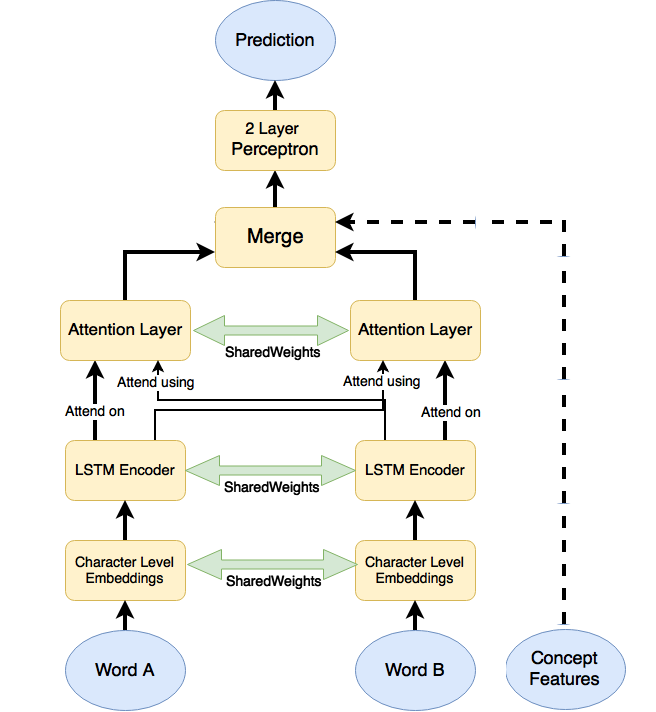
\includegraphics[width=0.45\textwidth]{CoAttNetwork}
    \caption{Recurrent Co-Attention Network for Cognate Discovery}
    \label{CoAttNet}
\end{figure}

The overall model used in our system is called the Recurrent Co-Attention Model (\textit{CoAtt}). It is adapted from the word-by-word attention model used by \citet{rocktaschel2016reasoning} for the task of recognising textual entailment (RTE) in natural language sentences. Just as the RTE task involves understanding the semantics of a sentence which is hidden behind sequence of words, the cognate identification task also requires information beyond surface character similarity, which was the motivation to adapt this particular model for our task. The network is illustrated in Figure~\ref{CoAttNet}. We have converted the RTE model into a siamese-style network that encodes a word pair in parallel and then makes a discriminative judgement in the final layer. 

The input words are first encoded into character level embeddings. Character embeddings are a form of distributional representation, where every character of the vocabulary is expressed as a vector in a vector space. Following the approach by \citet{rama2016siamese}, we define the character embeddings manually using various properties of the respective phoneme and then let these embeddings change during the training of the model, so that the representation is tuned for the task in hand. Initialising these embeddings to manually defined values rather than a random initialisation results in better training of the models.

The character encoded words are then further encoded using a bidirectional LSTM network. LSTMs or Long Short-Term Memory are a form of RNN and are extensively used in several NLP tasks. Finally the encoded words pass through a character by character attention layer. The attention layer essentially creates a weighted average of the sequence of vectors that represent a word coming out of the LSTM. The weights of the individual vectors in this average are computed dynamically depending on the characters present in the second word that it is being compared to. More intuitively, the attention mechanism helps to enhance the representation of a word obtained from the LSTM by giving it the `context' of the second word. The attended encodings of both the words are merged and passed to a 2-layer perceptron with \textit{tanh} and \textit{sigmoid} activations to make a binary prediction. 

Additionally, we also add a \textit{Concept features} vector to the model by concatenating it with the merged attention vector before passing it to the 2-layer neural network. We hypothesise that information regarding the semantics or the meaning of the input word pair should be helpful for the classification task. The word semantics can provide information like the POS category of the word, which can be useful if some POS classes show higher degree of variation in cognates than others. We implement this by using GloVe word embeddings \cite{pennington2014glove}. We use the GloVe embedding for the English concept of the word pair as obtained from the label in the dataset, and input this vector to the network. 

%%%%%%%%%%%%%%%%%%%%%%%%
\begin{table*}[t]
\centering

\begin{tabular}{lcccccc}
\multicolumn{1}{c}{\multirow{2}{*}{\textbf{Model}}} & \multicolumn{2}{l}{\textbf{Indo-European}}                              & \multicolumn{2}{c}{\textbf{Austronesian}} & \multicolumn{2}{c}{\textbf{Mayan}} \\ \cline{2-7} 
\multicolumn{1}{c}{}                                & \multicolumn{1}{l}{\textit{F-Score}} & \multicolumn{1}{l}{\textit{AUC}} & \textit{F-Score}      & \textit{AUC}      & \textit{F-Score}  & \textit{AUC}   \\ \hline
Gap-Weighted Subsequence                            & 59.0                                 & 75.5                             & 58.8                  & 68.9              & 71.8              & 81.8           \\
Phonetic CNN                                         & 73.7                                 & 86.1                             & 54.6                  & 68.0              & 72.8              & 85.0           \\
Character CNN                                        & 75.3                                 & 85.3                             & 62.2                  & 71.6              & 75.9              & 85.7           \\
LSTM + No Attention                                 & 56.7                                 & 59.0                             & 51.2                  & 55.2              & 60.6              & 67.1           \\
LSTM + Uniform Attention                            & 52.8                                 & 59.4                             & 49.8                  & 52.7              & 60.8              & 66.1           \\ \hline
Co-Attention Model                                  & 83.8                                 & 89.2                             & 69.0                  & 77.5              & 67.1              & 67.7           \\
\quad + IE                             & 85.1                                 & 92.4                             & 70.2                  & 79.3              & 63.6              & 71.3           \\
\quad + IE + CF                                  & \textbf{86.2}                                 & \textbf{93.0}                             & \textbf{70.5}         & \textbf{79.7}     & 81.5              & 89.0           \\
\quad + IE + PreT (Indo-European)                      & \textit{-}                           & \textit{-}                       & -                     & -                 & 82.5              & 90.6           \\
\quad + IE + PreT (Austronesian)                       & -                                    & -                                & -                     & -                 & \textbf{83.5}     & \textbf{91.2} 
\end{tabular}
\label{CL_res}
\caption{Cross Language Evaluation Results \newline [IE: \textit{Initialised Embeddings}, CF: \textit{Concept Features}, PreT: \textit{Pre-Training on another dataset}]}
\end{table*}
%%%%%%%%%%%%%%%%%%%%%%%%

%%%%%%%%%%%%%%%%%%%%%%%%%%%%%%%%%%%%%%%%%%%%%%%%
\section{Results}

%%%%%%%%%%%%%%%%%%%%%%%%
\subsection{Experimental Setting}

The task makes use of word lists of different language families taken from the basic vocabulary. A word list can be considered as a table where the different rows and columns represent different languages and concepts. Each cell in the table contains a lexical item along with its cognate class ID which helps to determine if two words are cognates. We worked with 3 language families in our experiments, namely Indo-European, Austronesian and Mayan. These families make a good test as they vary widely in terms of the number of languages, concepts and cognate classes.

We follow a Cross Language evaluation procedure, where the training and testing sample pairs are created using exclusive sets of languages. A random set of 70\% of the languages is set as the training set of languages and the rest as testing set. Both words in a sample pair belongs to the same concept or meaning. It must be noted that cognate words are not simply the translations of each other, but are known to have a common origin historically.

%%%%%%%%%%%%%%%%%%%%%%%%
\subsection{Evaluation Metric}

We report the \textit{F-score} and the area under the PR curve (\textit{AUC}) as a measure of performance for all the models. \textit{F-score} is computed as the harmonic mean of the \textit{precision} and \textit{recall}\footnote{Precision and Recall is computed on positive labels at 0.5 threshold. Precision = TP/(TP+FP), Recall = TP/(TP+FN)}. Since the dataset is heavily biased and contains a majority of negative cognate sample pairs, we do not use \textit{accuracy} as a measure of performance.

%%%%%%%%%%%%%%%%%%%%%%%%
\subsection{Baseline Models}

We compare against several baseline models. \textit{Gap-Weighted Subsequence} refers to the common subsequence model \cite{rama2015automatic} mentioned earlier. The \textit{Phonetic CNN} and \textit{Character CNN} models are reimplementations of the CNN-based models \cite{rama2016siamese}. We also introduced two sanity-check baseline models to test the attention layer of the \textit{CoAtt} model. The \textit{LSTM + No Attention} model removes the Co-Attention layer from the \textit{CoAtt} model, while the \textit{LSTM + Uniform Attention} model does a simple average rather than a weighted average in the attention layer.

%%%%%%%%%%%%%%%%%%%%%%%%
\subsection{Experiments with Indo-European}

We primarily worked with the Indo-European dataset on our experiments. As can be seen in Table 1, the \textit{CoAtt} model is clearly an improvement over the CNN and the subsequence based models. The \textit{LSTM + No Attention} and \textit{LSTM + Uniform Attention} models reflect the importance of the attention layer adapted from the RTE model in the network, as without it the model does not perform very good. 

A few additional features added to the \textit{CoAtt} model helps to improve it even further. Initialising the character embeddings with the manually defined vectors (\textit{IE} models) increases the \textit{AUC} by around 3\%. Further, addition of the \textit{Concept features} discussed earlier, is also found to be useful.

%%%%%%%%%%%%%%%%%%%%%%%%
\subsection{Experiments with Multiple Datasets}

We observe a similar trend for the models on the Austronesian and Mayan datasets as well. However, the \textit{CoAtt} model does not train well on the Mayan dataset directly. This poor performance on the Mayan dataset is associated with its small size. The Mayan dataset being significantly smaller than the other datasets, does not prove sufficient for training the \textit{CoAtt} network. We justify this hypothesis subsequently with the \textit{Cross-Family Pretraining} experiment. The \textit{Concept features} are again found useful to improve the \textit{CoAtt} model, especially on the Mayan dataset, where the extra information about the meaning of input word pair helps the model to cross the baseline results. 

%%%%%%%%%%%%%%%%%%%%%%
\subsubsection*{Cross Family Pre-training Experiments}

The three different language families with which we work have completely different origins and are placed across different regions geographically. We test if any notion of language evolution is still shared amongst these independently evolved families. This is done through the joint learning of models. The network is instantiated with the combined character vocabulary of two datasets. Then the model is trained on one dataset till the loss saturated. This is followed by the training on a second dataset, starting from the weights learned from the pre-training. 

It is found that such a joint-training procedure helps the \textit{CoAtt} model on the Mayan dataset significantly. The pretraining procedure is able to provide a good initialisation point to start training on the Mayan dataset. The pretrained models perform significantly better than the baseline models (\textit{PreT} models in Table 1). This also provides evidence to support our hypothesis that the \textit{CoAtt} was not able to learn on the Mayan dataset because of lack of enough data to train the network, but pre-training the model on other language families helped to show the true potential of the model on the dataset.

% %%%%%%%%%%%%%%%%%%%%%%%%%%%%%%%%%%%%%%%%%%%%%%%%
% \section{Analysis}

% \subsection{Concept Wise Performance}

% In this analysis of the models, we looked at the performance of various models over the individual concepts in the test set samples. It is observed that the performance of \textit{CoAtt} is more uniform throughout the concepts as compared to more varied distribution of the subsequence model. For concepts like WHAT, WHO, WHERE, HOW, THERE where the subsequence model performed poorly, the \textit{CoAtt} model is able to acheive high scores. The \textit{CoAtt} model performs poorly on a few selected concepts like AT, IF, IN, BECAUSE, GIVE. By looking at the samples, it is found that these concepts are heavily biased by negative samples and contain only a handful of positive cognate pair examples. In fact the subsequence model could not perform at all on these concepts as the highly biased data is coupled with almost no overlap of subsequences.

% \begin{table}[h]
% \centering
% \begin{tabular}{ccc}
% \textbf{Concept} & \textbf{CoAtt} & \textbf{Subseq} \\ \hline
% WHAT             & \textit{0.91}  & \textit{0.04}   \\
% WHO              & \textit{0.85}  & \textit{0.05}   \\
% WHERE            & \textit{0.90}  & \textit{0.16}   \\
% HOW              & \textit{0.90}  & \textit{0.17}   \\
% THERE            & \textit{0.95}  & \textit{0.19}  \\
% GIVE             & \textit{0.45}  & \textit{0.35}  \\
% BECAUSE          & \textit{0.28}  & \textit{0}      \\
% IN               & \textit{0.35}  & \textit{0}      \\
% IF               & \textit{0.31}  & \textit{0}      \\
% AT               & \textit{0.25}  & \textit{0}      
% \end{tabular}
% \caption{\textit{CoAtt} vs \textit{Subseq} model on various concepts (F-Score)}
% \end{table}

% \subsection{Transcription Tests}

% As mentioned in an earlier section, the Indo-European dataset is available to us different transcriptions. The dataset is trascribed in ASJP like the other datasets and is also transcribed in IPA, which is a much finer representation as compared to ASJP. On comparing the models trained on these different transcriptions of the same data, it is found that the IPA model performs poorly on some concepts like GUTS, SWIM, WIPE, WHITE, SING where the ASJP model gives good results. On the other hand, the IPA model performs relatively better on concepts like FIRE, SLEEP, PULL, SAY and SMOOTH. By looking at specific examples, we find that for concepts like FIRE and PULL, the ASJP model gives many false positives which can be a fault due to the coarser representation of the ASJP character.

% \begin{table}[h]
% \centering
% \begin{tabular}{ccc}
% \textbf{Concept} & \textbf{IPA}  & \textbf{ASJP} \\ \hline
% GUTS             & \textit{0.28} & \textit{0.58} \\
% SWIM             & \textit{0.47} & 0.93          \\
% WHITE            & \textit{0.54} & \textit{0.75} \\
% WIPE             & \textit{0.55} & \textit{0.72} \\
% SING             & \textit{0.56} & \textit{0.88} \\ \hline
% FIRE             & \textit{0.62} & \textit{0.33} \\
% SLEEP            & \textit{0.73} & 0.39          \\
% PULL             & \textit{0.83} & \textit{0.50} \\
% SMOOTH           & \textit{0.83} & \textit{0.50} \\
% SAY              & \textit{0.90} & \textit{0.51}
% \end{tabular}
% \caption{\textit{CoAtt} model using IPA vs ASJP transcription on various concepts (F-Score)}
% \end{table}

% \begin{figure}[t]
% \centering
%   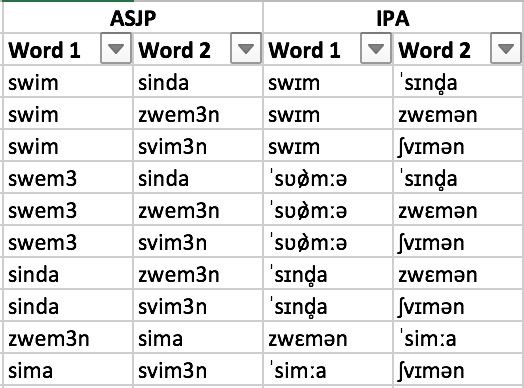
\includegraphics[width=.9\linewidth]{swim}
%   \caption{Sample test word pairs from the concept SWIM}
%   \label{disssim}
% \end{figure}

% Figure 2 shows few test sample pairs from the concept SWIM. It is observed that for all of these samples, the IPA model falsely predicts negatives whereas the ASJP model is correctly able to predict them all as cognates. Here perhaps the very find representation in IPA throws the model's judgment off and its not able to pick up the correspondence correctly. It is also interesting to note that for all of these samples, adding the \textit{concept feature} of SWIM to the \textit{CoAtt + Concept Features} model makes it predict all of them as cognates. Thus, perhaps adding the concept features signals the model to relax the degree of overlapping of phonemes and become less strict in predicting cognates.

% \subsection{Hindi-Marathi Domain Adaptation}

% Finally we applied the \textit{CoAtt} model to the domain of Hindi-Marathi. The model was trained on the IELex dataset with IPA transcription with a character vocabulary of around 150 phonetic characters. The model was trained in a cross-language evaluation style. It should be noted that the IELex database contains instances from Marathi, but it does not directly contain instances from Hindi. However, it does contain words from Urdu and Bhojpuri (Bihari) which are also languages closely related to Hindi and share many words of the vocabulary with Hindi.

% We used the TDIL sentence-aligned corpus. The corpus contains sentences from Hindi-Marathi that are POS tagged and transcribed in Devanagari. We specifically extracted word pairs from each sentence with the NOUN and VERB tags. Since the sentences are not word aligned, we extracted candidate word pairs for testing by choosing the first word with the same tag in either sentence as the candidate pair. The words were converted from Devanagari to IPA using a rule-based system and finally fed into the model. We extracted 16K pairs from Nouns and 9K pairs from Verbs.

% On first observation it seems that the model is doing a fair job of aligning similar word pairs that are possibly cognates. We tested the performance of the model by randomly sampling 50 word pairs each from NOUNs and VERBs and manually annotating them. We found that our model gives an 80\% accuracy on Verbs and 74\% accuracy on Nouns. The model is able to find word pairs with a common stem without the need of lemmetization. In the case of verbs, it can be observed that the model is able to see through the inflections on the verbs to predict the pairs with similar stems as cognates. 

%%%%%%%%%%%%%%%%%%%%%%%%%%%%%%%%%%%%%%%%%%%%%%%%
\section{Discussion}

The task of cognate discovery dwells into domain of finding rich hidden representation for words. It is found that simple surface similarity measures like common subsequence based features fail to capture the essence of phonological evolution and sound correspondences. Where there is large drift in the word structures and the characters of the words, these methods fail to capture any similarity between the words. Deep learning models like LSTMs are able to exploit hidden representations to make better judgments of word cognacy. 

Cognate formation results from the evolution of sound changes in the words over time. From our experiments we have seen that there is a link in this evolution of sound class with the semantics of the words. Because words with different meanings are used in different frequencies, some appear to go through rapid adaptation and while others do not change by a lot. The models generally perform better on Nouns and Adjective words and they also have more number of cognate classes. In particular, concepts like \textit{`WHAT'}, \textit{`WHEN'}, \textit{`HOW'} show a lot of variation even within a cognate class, so much that some cognate word pairs do not share any subsequence. Introducing concept features to the models in the form of word embeddings is seen to help in improving the results. It is also found that joint training of the models with data from different language families is also useful.

The task of discovering cognates can possibly be particularly useful among the languages of South Asia, which are not rich in lexical resources. Information about cognates can become an important source for assisting the creation and sharing of lexical resources between languages. By using DL models, the performance boosts are enough to test the model in an open domain. We applied our model to the domain of Hindi-Marathi, using a large unlabelled corpus of aligned texts to find cognate pairs and found through manual evaluation that the model is able to segregate the word pairs efficiently. 

%%%%%%%%%%%%%%%%%%%%%%%%%%%%%%%%%%%%%%%%%%%%%%%%
\bibliography{emnlp2017}

\bibliographystyle{emnlp_natbib}

\end{document}
